% !TeX program = xelatex
\documentclass{article}
\usepackage{kotex}
\usepackage[a4paper,left=3cm, right=3cm, top=2cm, bottom=2cm]{geometry}
\usepackage{amsmath}
\usepackage{graphicx}
\usepackage{caption}
\usepackage{setspace}
\usepackage{xcolor}
\usepackage{titlesec}
\usepackage{amssymb}
\usepackage{tcolorbox}
\usepackage{wrapfig}
\usepackage{amsthm}
\usepackage{multirow} 
\usepackage{array}
\usepackage{tcolorbox}
\usepackage{pgfplots}
\pgfplotsset{compat=1.18} % For proofs

\graphicspath{{graph/}}
\title{7.1 곡면의 종류}
\date{}
\author{}
\setstretch{1.3}

% \subsection* 형식 지정 (번호 없음)
\titleformat{name=\section, numberless}
  {\normalfont\large\bfseries\color{blue}}
  {}
  {0pt}
  {}
\geometry{a4paper, margin=1in}

% 증명 환경 스타일
\newtheoremstyle{mystyle}% name
  {}% Space above
  {}% Space below
  {\itshape}% Body font
  {}% Indent amount
  {\bfseries}% Theorem head font
  {.}% Punctuation after theorem head
  {.5em}% Space after theorem head
  {}% Theorem head spec (can be left empty, meaning `normal')
\theoremstyle{mystyle}

\begin{document}
\maketitle

\begin{tcolorbox}[colback=blue!5, colframe=blue!60!black, title=7.2 이차곡면 -- 한눈에 보기, boxrule=0.5mm, arc=3mm]
\begin{center}
\renewcommand{\arraystretch}{1.3}
\begin{tabular}{|p{2.5cm}|p{6cm}|p{5.5cm}|}
\hline
\textbf{종류} & \textbf{표준형} & \textbf{특징} \\
\hline
타원면 & $\dfrac{x^2}{a^2}+\dfrac{y^2}{b^2}+\dfrac{z^2}{c^2}=1$ & 중심 원점, 세 축 모두 닫힌 타원 단면 \\
\hline
일엽쌍곡면 & $\dfrac{x^2}{a^2}+\dfrac{y^2}{b^2}-\dfrac{z^2}{c^2}=1$ & 한 조각(연결됨), 축 방향 단면은 쌍곡선 \\
\hline
이엽쌍곡면 & $\dfrac{x^2}{a^2}-\dfrac{y^2}{b^2}-\dfrac{z^2}{c^2}=1$ & 두 조각으로 분리 \\
\hline
타원포물면 & $\dfrac{x^2}{a^2}+\dfrac{y^2}{b^2}=z$ & 꼭짓점 하나, 밥그릇 모양 \\
\hline
쌍곡포물면 & $\dfrac{x^2}{a^2}-\dfrac{y^2}{b^2}=z$ & 안장 모양, $z=0$에서 두 직선 \\
\hline
\end{tabular}
\end{center}
\end{tcolorbox}

이차방정식
\[
ax^2+by^2+cz^2+2fyz+2gzx+2hxy+2lx+2my+2nz+d=0
\]
의 그래프를 \textbf{이차곡면}이라 한다. 이차곡면에는 어떤 종류가 있는지 알아보자.

\section*{[1] 타원면 (Ellipsoid)}

\begin{tcolorbox}[
    colback=teal!4,
    colframe=teal!65!black,
    title=정의 \& 핵심 규칙,
    fonttitle=\bfseries,
    boxrule=0.5mm,
    arc=3mm
    ]
    \textbf{\textcolor{teal!65!black}{정의.}}\quad
    방정식
    \[
    \frac{x^2}{a^2}+\frac{y^2}{b^2}+\frac{z^2}{c^2}=1 \tag{1}
    \]
    이 표시하는 곡면을 \textbf{타원면}이라 한다.

    \noindent\textcolor{teal!50!black}{\rule{\linewidth}{0.4pt}}

    \textbf{\textcolor{teal!65!black}{핵심 규칙.}}\quad
    중심은 원점이고, 꼭짓점의 좌표는 \((\pm a,0,0),\ (0,\pm b,0),\ (0,0,\pm c)\)이며, 주축의 길이는 각각 \(2a,2b,2c\)이다. 방정식 (1)을 \textbf{타원면의 표준형}이라 한다.
\end{tcolorbox}
\begin{figure}[h]
\centering
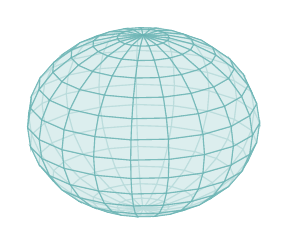
\begin{tikzpicture}
\begin{axis}[hide axis, view={115}{20}, width=5.5cm, height=5.5cm]
\addplot3[
    surf, shader=faceted, faceted color=teal!60, fill=teal!15, opacity=0.7,
    domain=0:180, domain y=0:360, samples=15, samples y=20, z buffer=sort,
]
({2*sin(x)*cos(y)}, {1.2*sin(x)*sin(y)}, {1.5*cos(x)});
\end{axis}
\end{tikzpicture}
\caption{타원면 $\frac{x^2}{a^2}+\frac{y^2}{b^2}+\frac{z^2}{c^2}=1$}
\end{figure}

타원면 (1)과 각 좌표면과의 교선은 다음과 같다.

\begin{center}
\renewcommand{\arraystretch}{1.4}
\begin{tabular}{|l|l|}
\hline
좌표평면 & 교선 \\
\hline
\(xy\)평면 & \(\dfrac{x^2}{a^2}+\dfrac{y^2}{b^2}=1\) \\
\hline
\(zx\)평면 & \(\dfrac{x^2}{a^2}+\dfrac{z^2}{c^2}=1\) \\
\hline
\(yz\)평면 & \(\dfrac{y^2}{b^2}+\dfrac{z^2}{c^2}=1\) \\
\hline
\end{tabular}
\end{center}

그리고 \(|k|<c\)인 모든 \(k\)에 대하여 \(z=k\)인 평면으로 타원면 (1)을 자르면 잘린 부분은 다음과 같은 타원이다.
\[
\frac{x^2}{a^2\left(1-\dfrac{k^2}{c^2}\right)}+\frac{y^2}{b^2\left(1-\dfrac{k^2}{c^2}\right)}=1
\]

\subsection*{EXAMPLE 1}
일직선 위의 세 정점 \(A,B,C\)가 각각 \(yz,zx,xy\)평면 위에 있도록 움직일 때, 그 직선 위의 제4의 정점 \(P\)가 그리는 자취를 구하여라.\\
\textbf{SOLUTION:}
\(\overline{PA}=a,\overline{PB}=b,\overline{PC}=c\)라 두고 \(P\)의 좌표를 \((x,y,z)\)라 하자. 직선의 방향코사인을 \(\lambda,\mu,\nu\)라 하면
\[
A(x+\lambda a,\ y+\mu a,\ z+\nu a),\quad B(x+\lambda b,\ y+\mu b,\ z+\nu b),\quad C(x+\lambda c,\ y+\mu c,\ z+\nu c)
\]
이다. \(A,B,C\)는 각각 \(yz,zx,xy\)평면 위에 있으므로
\[
x+\lambda a=0,\qquad y+\mu b=0,\qquad z+\nu c=0
\]
이고, \(\lambda^2+\mu^2+\nu^2=1\)에서 \(\lambda,\mu,\nu\)를 소거하면
\[
\frac{x^2}{a^2}+\frac{y^2}{b^2}+\frac{z^2}{c^2}=1
\]
따라서 구하는 자취는 \textbf{타원면}이다.

\section*{[2] 쌍곡면 (Hyperboloid)}

\subsection*{(i) 일엽쌍곡면}

\begin{tcolorbox}[
    colback=teal!4,
    colframe=teal!65!black,
    title=정의 \& 핵심 규칙,
    fonttitle=\bfseries,
    boxrule=0.5mm,
    arc=3mm
    ]
    \textbf{\textcolor{teal!65!black}{정의.}}\quad
    방정식
    \[
    \frac{x^2}{a^2}+\frac{y^2}{b^2}-\frac{z^2}{c^2}=1 \tag{2}
    \]
    이 표시하는 곡면을 \textbf{일엽쌍곡면}이라 하고, 원점과 \(z\)축을 각각 이 곡면의 중심과 축이라 한다.

    \noindent\textcolor{teal!50!black}{\rule{\linewidth}{0.4pt}}

    \textbf{\textcolor{teal!65!black}{핵심 규칙.}}\quad
    부호가 \((+,+,-)\)이면 \textbf{한 조각으로 연결된} 쌍곡면이다 (마이너스 부호가 하나뿐).
\end{tcolorbox}

\begin{figure}[h]
\centering
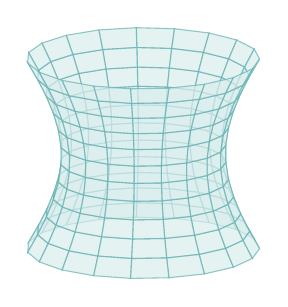
\begin{tikzpicture}
\begin{axis}[hide axis, view={115}{15}, width=5.5cm, height=5.5cm]
\addplot3[
    surf, shader=faceted, faceted color=teal!60, fill=teal!15, opacity=0.7,
    domain=-1:1, domain y=0:360, samples=12, samples y=20, z buffer=sort,
]
({1.3*sqrt(1+x^2)*cos(y)}, {1.3*sqrt(1+x^2)*sin(y)}, {2*x});
\end{axis}
\end{tikzpicture}
\caption{일엽쌍곡면 -- 한 조각으로 연결}
\end{figure}


좌표면과의 교선은 다음과 같다.

\begin{center}
\renewcommand{\arraystretch}{1.4}
\begin{tabular}{|l|l|l|}
\hline
좌표평면 & 교선 & 종류 \\
\hline
\(xy\)평면 & \(\dfrac{x^2}{a^2}+\dfrac{y^2}{b^2}=1\) & 타원 \\
\hline
\(zx\)평면 & \(\dfrac{x^2}{a^2}-\dfrac{z^2}{c^2}=1\) & 쌍곡선 \\
\hline
\(yz\)평면 & \(\dfrac{y^2}{b^2}-\dfrac{z^2}{c^2}=1\) & 쌍곡선 \\
\hline
\end{tabular}
\end{center}

임의의 \(k\)에 대하여 평면 \(z=k\)로 자르면 잘린 부분은 타원
\[
\frac{x^2}{a^2\left(1+\dfrac{k^2}{c^2}\right)}+\frac{y^2}{b^2\left(1+\dfrac{k^2}{c^2}\right)}=1
\]
이고, \(|h|<b\)인 \(h\)에 대하여 평면 \(y=h\)로 자르면 잘린 부분은 다음과 같은 쌍곡선이다.
\[
\frac{z^2}{a^2\left(1-\dfrac{h^2}{b^2}\right)}-\frac{y^2}{c^2\left(1-\dfrac{h^2}{b^2}\right)}=1
\]

\subsection*{EXAMPLE 2}
\(x^2-y^2+2z^2-4x-6y-8z-3=0\)이 표시하는 곡면은 무엇인가?\\
\textbf{SOLUTION:} 주어진 방정식을 변형하면
\[
\frac{(x-2)^2}{6}-\frac{(y+3)^2}{6}+\frac{(z-2)^2}{3}=1
\]
즉, 이 곡면은 중심이 \((2,-3,2)\)이고, 축이 \(zx\)평면에 수직인 \textbf{일엽쌍곡면}이다.

\subsection*{(ii) 이엽쌍곡면}

\begin{tcolorbox}[
    colback=teal!4,
    colframe=teal!65!black,
    title=정의 \& 핵심 규칙,
    fonttitle=\bfseries,
    boxrule=0.5mm,
    arc=3mm
    ]
    \textbf{\textcolor{teal!65!black}{정의.}}\quad
    방정식
    \[
    \frac{x^2}{a^2}-\frac{y^2}{b^2}-\frac{z^2}{c^2}=1 \tag{3}
    \]
    으로 표시된 곡면을 \textbf{이엽쌍곡면}이라 한다.

    \noindent\textcolor{teal!50!black}{\rule{\linewidth}{0.4pt}}

    \textbf{\textcolor{teal!65!black}{핵심 규칙.}}\quad
    부호가 \((+,-,-)\)이면 \textbf{두 조각으로 분리된} 쌍곡면이다 (마이너스 부호가 둘). \(|k|\ge a\)인 \(k\)에 대해서만 평면 \(x=k\)와 만난다.
\end{tcolorbox}

\begin{figure}[h]
\centering
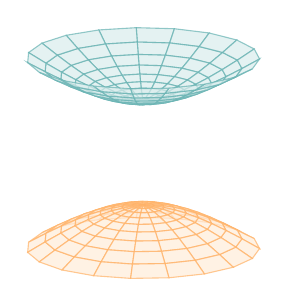
\begin{tikzpicture}
\begin{axis}[hide axis, view={115}{15}, width=5.5cm, height=5.5cm]
\addplot3[
    surf, shader=faceted, faceted color=teal!60, fill=teal!15, opacity=0.7,
    domain=0:1.2, domain y=0:360, samples=10, samples y=20, z buffer=sort,
]
({1.3*sinh(x)*cos(y)}, {1.3*sinh(x)*sin(y)}, {2*cosh(x)});
\addplot3[
    surf, shader=faceted, faceted color=orange!60, fill=orange!15, opacity=0.7,
    domain=0:1.2, domain y=0:360, samples=10, samples y=20, z buffer=sort,
]
({1.3*sinh(x)*cos(y)}, {1.3*sinh(x)*sin(y)}, {-2*cosh(x)});
\end{axis}
\end{tikzpicture}
\caption{이엽쌍곡면 -- 두 조각으로 분리}
\end{figure}

\(|k|\ge a\)인 \(k\)에 대하여 평면 \(x=k\)로 자르면 잘린 부분은 타원
\[
\frac{y^2}{b^2\left(\dfrac{k^2}{a^2}-1\right)}+\frac{z^2}{c^2\left(\dfrac{k^2}{a^2}-1\right)}=1
\]
이고, 좌표면과의 교선은 다음과 같다.

\begin{center}
\renewcommand{\arraystretch}{1.4}
\begin{tabular}{|l|l|l|}
\hline
좌표평면 & 교선 & 종류 \\
\hline
\(xy\)평면 & \(\dfrac{x^2}{a^2}-\dfrac{y^2}{b^2}=1\) & 쌍곡선 \\
\hline
\(zx\)평면 & \(\dfrac{x^2}{a^2}-\dfrac{z^2}{c^2}=1\) & 쌍곡선 \\
\hline
\end{tabular}
\end{center}

\section*{[3] 포물면 (Paraboloid)}

\subsection*{(i) 타원포물면}

\begin{tcolorbox}[
    colback=teal!4,
    colframe=teal!65!black,
    title=정의 \& 핵심 규칙,
    fonttitle=\bfseries,
    boxrule=0.5mm,
    arc=3mm
    ]
    \textbf{\textcolor{teal!65!black}{정의.}}\quad
    방정식
    \[
    \frac{x^2}{a^2}+\frac{y^2}{b^2}=z
    \]
    로 표시되는 곡면을 \textbf{타원포물면}이라 한다.

    \noindent\textcolor{teal!50!black}{\rule{\linewidth}{0.4pt}}

    \textbf{\textcolor{teal!65!black}{핵심 규칙.}}\quad
    \(z\)가 일차식이고 \(x^2,y^2\) 부호가 \textbf{같으면} 타원포물면(밥그릇 모양)이다. \(xy\)평면과는 원점에서만 만나며, 이 점을 \textbf{꼭짓점}이라 한다.
\end{tcolorbox}

\begin{figure}[h]
\centering
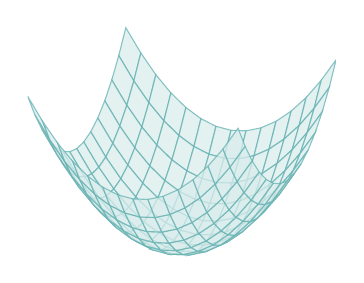
\begin{tikzpicture}
\begin{axis}[hide axis, view={115}{20}, width=5.5cm, height=5.5cm]
\addplot3[
    surf, shader=faceted, faceted color=teal!60, fill=teal!15, opacity=0.75,
    domain=-1.4:1.4, domain y=-1.4:1.4, samples=15, samples y=15,
]
{x^2+y^2};
\end{axis}
\end{tikzpicture}
\caption{타원포물면 -- 밥그릇 모양}
\end{figure}

\(k>0\)인 \(k\)에 대하여 평면 \(z=k\)로 자르면 잘린 부분은 타원 \(\dfrac{x^2}{a^2}+\dfrac{y^2}{b^2}=k\)이고, \(|h|\le b\)인 \(h\)에 대하여 평면 \(y=h\)로 자르면 잘린 부분은 포물선 \(x^2=a^2z-\dfrac{a^2h^2}{b^2}\)이다. 좌표면과의 교선은 다음과 같다.

\begin{center}
\renewcommand{\arraystretch}{1.4}
\begin{tabular}{|l|l|l|}
\hline
좌표평면 & 교선 & 종류 \\
\hline
\(zx\)평면 & \(x^2=a^2z\) & 포물선 \\
\hline
\(yz\)평면 & \(y^2=b^2z\) & 포물선 \\
\hline
\(xy\)평면 & 원점에서만 만남 (꼭짓점) & --- \\
\hline
\end{tabular}
\end{center}

\subsection*{EXAMPLE 3}
\(x^2+2z^2-3x-2z-y+\dfrac{5}{2}=0\)이 표시하는 곡면은 무엇인가?\\
\textbf{SOLUTION:} 주어진 방정식을 변형하면
\[
\left(x-\frac{3}{2}\right)^2+2\left(z-\frac{1}{2}\right)^2=y+\frac{1}{4}
\]
즉, 이 곡면은 꼭짓점이 \(\left(\dfrac{3}{2},-\dfrac{1}{4},\dfrac{1}{2}\right)\)이고, \(y\)축의 양의 방향으로 벌어져 있는 \textbf{타원포물면}이다.

\subsection*{(ii) 쌍곡포물면}

\begin{tcolorbox}[
    colback=teal!4,
    colframe=teal!65!black,
    title=정의 \& 핵심 규칙,
    fonttitle=\bfseries,
    boxrule=0.5mm,
    arc=3mm
    ]
    \textbf{\textcolor{teal!65!black}{정의.}}\quad
    방정식
    \[
    \frac{x^2}{a^2}-\frac{y^2}{b^2}=z
    \]
    로 표시되는 곡면을 \textbf{쌍곡포물면}이라 한다.

    \noindent\textcolor{teal!50!black}{\rule{\linewidth}{0.4pt}}

    \textbf{\textcolor{teal!65!black}{핵심 규칙.}}\quad
    \(z\)가 일차식이고 \(x^2,y^2\) 부호가 \textbf{다르면} 쌍곡포물면(안장 모양)이다. \(z=0\)과의 교선은 \textbf{두 직선}이다.
\end{tcolorbox}

\begin{figure}[h]
\centering
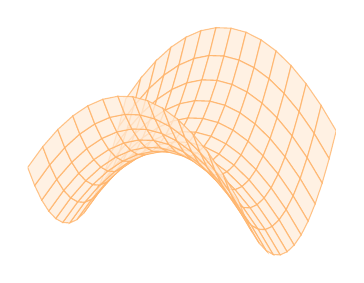
\begin{tikzpicture}
\begin{axis}[hide axis, view={115}{20}, width=5.5cm, height=5.5cm]
\addplot3[
    surf, shader=faceted, faceted color=orange!60, fill=orange!15, opacity=0.75,
    domain=-1.4:1.4, domain y=-1.4:1.4, samples=15, samples y=15,
]
{x^2-y^2};
\end{axis}
\end{tikzpicture}
\caption{쌍곡포물면 -- 안장 모양}
\end{figure}

이 곡면과 두 평면 \(x=0,\ y=0\)과의 교선은 각각 포물선 \(y^2=-b^2z,\ x^2=a^2z\)이고, 평면 \(z=k\ (k\ne0)\)와의 교선은 쌍곡선 \(\dfrac{x^2}{a^2k}-\dfrac{y^2}{b^2k}=1\)이다. 평면 \(z=0\)과의 교선은
\[
\frac{x^2}{a^2}-\frac{y^2}{b^2}=0 \quad\text{즉,}\quad \frac{y}{b}=\pm\frac{x}{a}
\]
인 \textbf{두 개의 직선}이다.

\subsection*{EXAMPLE 4}
쌍곡포물면 \(\dfrac{x^2}{4}-\dfrac{y^2}{9}=z\)가 평면 \(y=3\)과 만나는 포물선의 초점의 좌표를 구하여라.\\
\textbf{SOLUTION:} \(y=3\)을 대입하면
\[
\frac{x^2}{4}=z+1 \quad\text{즉,}\quad x^2=4\times1\times(z+1)
\]
따라서 초점의 좌표는 \((0,3,1-1)\) 즉, \(\boldsymbol{(0,3,0)}\)이다.

\begin{tcolorbox}[
    colback=red!4,
    colframe=red!60!black,
    title=이차곡면 판별 요약,
    fonttitle=\bfseries,
    boxrule=0.5mm,
    arc=3mm
    ]
    \(\pm\dfrac{x^2}{a^2}\pm\dfrac{y^2}{b^2}\pm\dfrac{z^2}{c^2}=1\) 꼴에서 마이너스 부호의 개수로, \(\pm\dfrac{x^2}{a^2}\pm\dfrac{y^2}{b^2}=z\) 꼴에서 부호의 일치 여부로 곡면이 결정된다.
\end{tcolorbox}

\begin{center}
\renewcommand{\arraystretch}{1.4}
\begin{tabular}{|l|l|}
\hline
부호 패턴 & 곡면 \\
\hline
\((+,+,+)=1\) & 타원면 \\
\hline
\((+,+,-)=1\) & 일엽쌍곡면 (한 조각) \\
\hline
\((+,-,-)=1\) & 이엽쌍곡면 (두 조각) \\
\hline
\((+,+)=z\) (부호 같음) & 타원포물면 \\
\hline
\((+,-)=z\) (부호 다름) & 쌍곡포물면 (안장) \\
\hline
\end{tabular}
\end{center}

\section*{연습문제 7.2}
\begin{enumerate}
    \item 다음 방정식들이 표시하는 곡면은 무엇인가?
    \begin{enumerate}
        \item[(1)] \(6x^2+3y^2+2z^2-6y-3=0\)
        \item[(2)] \(2x^2-y^2-2z^2-4y-6=0\)
    \end{enumerate}
    \item 다음과 같은 점의 자취를 구하여라.
    \begin{enumerate}
        \item[(1)] 점 \((2,1,-1)\)로부터의 거리가 \(y\)축으로부터의 거리의 3배인 점
        \item[(2)] 점 \((1,0,0)\)으로부터의 거리가 점 \((-1,0,0)\)으로부터의 거리에 1을 더한 것과 같은 점
    \end{enumerate}
\end{enumerate}
\end{document}